\documentclass{beamer}

\usepackage{fontspec,xunicode,xltxtra}

\XeTeXlinebreaklocale "zh"
\XeTeXlinebreakskip = 0pt plus 1pt minus 0.1pt

%\setmainfont[Mapping=tex-text]{AR PL UMing CN:style=Light}
%\setmainfont[Mapping=tex-text]{AR PL UKai CN:style=Book}
%\setmainfont[Mapping=tex-text]{WenQuanYi Zen Hei:style=Regular}
%\setmainfont[Mapping=tex-text]{WenQuanYi Zen Hei Sharp:style=Regular}
%\setmainfont[Mapping=tex-text]{AR PL KaitiM GB:style=Regular} 
%\setmainfont[Mapping=tex-text]{AR PL SungtiL GB:style=Regular} 
%\setmainfont[Mapping=tex-text]{WenQuanYi Zen Hei Mono:style=Regular} 

\newfontfamily\hei{WenQuanYi Micro Hei}
\newfontfamily\whei{WenQuanYi Zen Hei}
\newfontfamily\kai{AR PL UKai CN}
\newfontfamily\song{AR PL UMing CN}
\newfontfamily\bhei{cwTeXHeiBold}
%\newfontfamily\lishu{SIMLI}
\setmainfont[Mapping=tex-text]{WenQuanYi Micro Hei}
\setsansfont[Mapping=tex-text]{AR PL UKai CN}
\setmonofont[Mapping=tex-text]{WenQuanYi Zen Hei Mono}

\renewcommand{\baselinestretch}{1.25}


\mode<presentation>
{
  \usetheme{Warsaw}
  % or ...
  %\usetheme{default}

  \setbeamercovered{transparent}
  % or whatever (possibly just delete it)
}


\usepackage[english]{babel}
\usepackage{graphicx}
\usepackage{fontspec}


\title{最小二乘拟合}
\author{你的名字}
\date{\today}

\begin{document}

\begin{frame}
  \titlepage
\end{frame}

\begin{frame}{介绍}
  最小二乘拟合是一种数学方法,用于寻找最佳拟合曲线或直线,使得观测数据点与预测值之间的平方差之和最小化。

  \begin{figure}
    \centering
    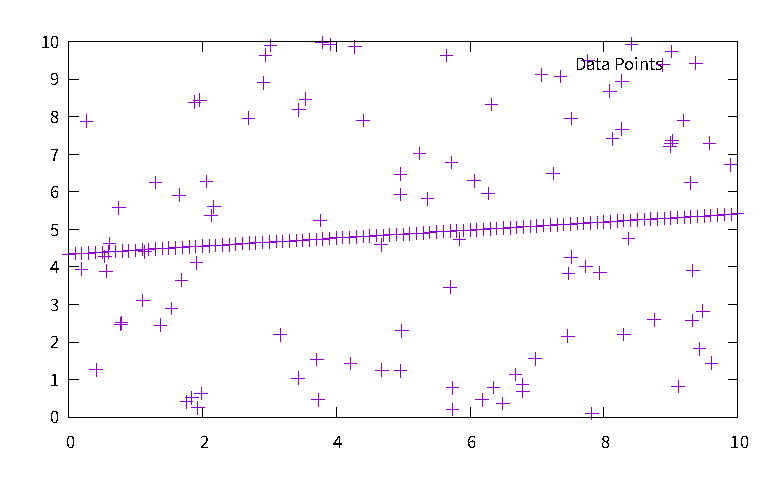
\includegraphics[width=0.6\textwidth]{output.eps}
    \caption{最小二乘拟合}
    \label{fig:fitting}
  \end{figure}
\end{frame}

\begin{frame}{拟合方法}
  在最小二乘拟合中,我们通过最小化观测数据点与拟合值之间的平方差来找到最佳拟合直线或曲线。

  \begin{itemize}
    \item 步骤 1: 收集观测数据点。
    \item 步骤 2: 选择适当的拟合函数形式。
    \item 步骤 3: 计算拟合函数的参数,使得平方差之和最小化。
  \end{itemize}
\end{frame}

\begin{frame}{最小二乘拟合公式}
  最小二乘拟合的目标是找到最佳拟合参数 $\mathbf{w}$,使得观测数据点与拟合值之间的平方差最小化。

  假设有 $n$ 个观测数据点 $(x_i, y_i)$,拟合函数的形式为 $y = f(x, \mathbf{w})$,其中 $\mathbf{w} = (w_0, w_1, \ldots, w_m)$ 是拟合函数的参数。

  平方差之和可以表示为:
  \[
  S(\mathbf{w}) = \sum_{i=1}^{n} (y_i - f(x_i, \mathbf{w}))^2
  \]

  最小二乘拟合的目标是找到使 $S(\mathbf{w})$ 最小的参数 $\mathbf{w}$。

  为了实现最小化,可以通过求解下面的方程组获得最佳参数 $\mathbf{w}$:
  \[
  \frac{\partial S(\mathbf{w})}{\partial w_j} = 0, \quad j = 0, 1, \ldots, m
  \]

  解得的参数 $\mathbf{w}$ 即为最小二乘拟合的结果。
\end{frame}

\begin{frame}{结论}
  最小二乘拟合是一种常用的数学方法,用于找到最佳拟合曲线或直线,以尽可能准确地拟合给定的观测数据点。

  \begin{itemize}
    \item 可以通过最小化观测数据点与拟合值之间的平方差来获得最佳拟合。
    \item 最小二乘拟合在多个领域都有广泛的应用,例如统计学、工程学和数据分析等。
  \end{itemize}
\end{frame}

\end{document}
